% Preamble
\pdfminorversion=4
\documentclass[aspectratio=169,xcolor=table]{beamer}
\usepackage{colortbl}
\usepackage{multimedia} % for videos
\usepackage{bm} % for bold math (for tensors)
\usepackage{layout} % put command \layout{} onto an empty frame to see margin lengths
\usepackage[export]{adjustbox}
\usepackage{lipsum}
\usepackage{pdfpages}
\usepackage{hyperref} % for hyperlinks
\usepackage{ulem} % for underline, etc.
\usepackage{array} % for table spacing
\usepackage{animate} % for animategraphics

% ----- beamer settings -----
% {{{

% define some colors/shades
\definecolor{lightblue}{HTML}{66A3D2}
\definecolor{darkblue}{HTML}{0B61A4}
\definecolor{usfgold}{HTML}{CFC493}
\definecolor{usfgreen}{HTML}{006747}
\definecolor{lightorange}{HTML}{FF8E0B}
\definecolor{darkorange}{HTML}{D45500}
\definecolor{paleorange}{HTML}{FFDEB3}
\definecolor{FigPurple}{HTML}{985277}

% set color for hyperlinks
\hypersetup{colorlinks=true, linkcolor=darkgray, citecolor=darkgray, urlcolor=darkgray}

% set theme
\usetheme{boxes}
\usefonttheme[onlymath]{serif}

% set beamer theme colors, etc.
\setbeamercolor{frametitle}{fg=black}

% customize blocks
\setbeamertemplate{blocks}[rounded][shadow=false]
\setbeamercolor{block title}{fg=white, bg=usfgreen}
\setbeamercolor{block body}{fg=black, bg=usfgold}

% customize enumerate and item, including color and spacing
\setbeamercolor*{item}{fg=usfgreen}
\setbeamercolor*{enumerate item}{fg=black}
\setbeamercolor*{enumerate subitem}{fg=black}
\setbeamercolor*{enumerate subsubitem}{fg=black}
\setbeamertemplate{itemize subitem}{$-$}
\setlength{\leftmarginii}{10pt}
\newlength\origleftmargini
\setlength\origleftmargini\leftmargini

% customize footer
\setbeamercolor{footline}{fg=gray}
\setbeamertemplate{navigation symbols}{} % get rid of navigation bar

% add page numbers to footer
\makeatletter
\setbeamertemplate{footline}{
    \leavevmode%
    \hbox{%
    \begin{beamercolorbox}[wd=0.5\paperwidth,ht=2.25ex,dp=1ex,left,leftskip=1ex]{}
    \end{beamercolorbox}
    \begin{beamercolorbox}[wd=0.5\paperwidth,ht=2.25ex,dp=1ex,right,rightskip=2ex]{}
      \insertframenumber % page number only
      % \insertframenumber/\inserttotalframenumber % page number/total pages
    \end{beamercolorbox}
    }\vskip0pt
}
\makeatother
% }}}

% ----- tikz ----- (for drawing)
% {{{
\usepackage{tikz}
\usetikzlibrary{shapes,positioning,arrows,backgrounds,fit}
% tikz define invisible: 
% http://tex.stackexchange.com/questions/55806/mindmap-tikzpicture-in-beamer-reveal-step-by-step/55849#55849
\tikzset{
  invisible/.style={opacity=0.2},
  visible on/.style={alt=#1{}{invisible}},
  alt/.code args={<#1>#2#3}{%
    \alt<#1>{\pgfkeysalso{#2}}{\pgfkeysalso{#3}} % \pgfkeysalso doesn't change the path
  },
}

\pgfdeclarelayer{bg}    % declare background layer
\pgfsetlayers{bg,main}  % set the order of the layers (main is the standard layer)

\newcommand{\highlighteq}[2]{ \tikz[baseline]{\node[fill=#1,rounded corners,anchor=base]{$\displaystyle \strut #2$};} }

\tikzset{onslide/.code args={<#1>#2}{%
  \only<#1>{\pgfkeysalso{#2}} % \pgfkeysalso doesn't change the path
}}

% }}}

% --- Notes on options for including movies ---
% {{{

% (1) movie15 package
% \usepackage{movie15}
% \includemovie[text={\includegraphics[width=5cm]{figs/lam_t0.pdf}}]{}{}{figs/lam.avi}
% Comments: 
%   * apparently depreciated (superceded by movie9), but seems to play movies fine
%   * (bad) Puts a pushpin icon over the video
%   * (good) Actually embeds the movie, so don't need to include a separate folder
%   * (bad) Puts black or white bars when playing movie with controls (changes size of
%     the movie to fit the controls into the frame).

% (2) movie9 package
% \usepackage{media9}
% Comments:
%   * Plays using a flash player. Doesn't work on Linux.

% (3) multimedia package
% \usepackage{multimedia}
% \movie[width=5cm, showcontrols]{\includegraphics[width=5cm]{figs/lam_t0.pdf}}{figs/lam.avi}
% Comments:
%   * (good) Seems like the best (but flawed) option for playing a movie in the frame
%   * (bad) Does not embed the movie. Need a separate videos folder.
%   * (bad) Puts black or white bars when playing movie with controls (changes size of
%     the movie to fit the controls into the frame).
%   * (aside) Appears that the backend of the player (same as movie15 pacakge) can be 
%     changed from gstreamer to vlc. Used apt-get install phonon-backend-vlc. Made bars
%     white, not black, which was a marginal improvement.
%     http://tex.stackexchange.com/questions/163089/okular-to-play-embedded-videos-in-beamer

% (4) Hyperlink
% \include{hyperref}
% \href{run:figs/lam.avi}{\includegraphics[width=5cm]{figs/lam_t0.pdf}}
% Comments:
%   * Runs an external viewer (like VLC)
%   * (good) Cross-platform compatible
%   * (bad) Means lots of clicking, and not very easy to move back and forth
%   * (bad) Does not embed the movie. Need a separate videos folder.
%   * (bad) Cannot set up a script to give arguments to external program (e.g. VLC)

% (5) pdfpc
% \href{run:figs/lam.avi?autostart&loop}{\includegraphics[width=5cm]{figs/lam_t0.pdf}}
% Comments:
%   * (neutral) Separate presentation platform. Has nice features.
%   * (bad) Has a slow "pre-rendering" feature.
%   * (bad) All tested videos end up very poor resolution.
%   * (good) Viewer does not re-size videos with ugly controls

% }}}

% ----- tips/tricks & custom definitions ----
% {{{

%% ** block title without a block **
\newcommand{\blocktitle}[1]{
  \begin{tikzpicture}
    \node[ fill, color=usfgreen, text=white, rounded corners, inner sep=4pt,
           align=center, minimum width=3cm, minimum height=\baselineskip
    ] 
    {\large #1\par};
  \end{tikzpicture}
}

% ** columns **
%  \begin{columns}[T]
%    \begin{column}{0.45\textwidth}
%      Column 1: Theory
%    \end{column}
%    \begin{column}{0.45\textwidth}
%      Column 2: Experiment
%    \end{column}
%  \end{columns}

% ** make a figure bigger than the textwidth **
%\makebox[\textwidth][c]{\includegraphics[width=1.0\textwidth]{figs/immersion_precipitation_roll.pdf}}

% ** bulk commenting **
%\iffalse
%\fi

% ** Put citation in bottom middle **
%\begin{tikzpicture}[remember picture, overlay]
%  \node[text width=\textwidth, align=center, anchor=south] at (current page.south) {
%    \scriptsize Lee et al. Adv.~Materials. 29, 1076008 (2017)\par
%  };
%\end{tikzpicture}

% }}}

% custom title page
% {{{
\setbeamerfont{author}{size=\normalsize} % font sizes
\newcommand{\location}[1]{\def\insertlocation{#1}}
\newcommand{\titlecolor}{\color{white}}
\newcommand{\bottomcolor}{\color{white}}
% https://tex.stackexchange.com/questions/350511/latex-beamer-create-own-variable
\newcommand\insertpresenter{}
\newcommand\presenter[1]{\renewcommand\insertpresenter{ \uline{#1}} }

\defbeamertemplate*{title page}{customized}[1][]
{
    \begin{tikzpicture}[remember picture, overlay]

      % background photo
      \node [draw=none, align=center] at (current page.center)
      {
        \includegraphics[keepaspectratio, width=1.01\paperwidth]{./figs/Background_image.jpg}
      };

      % USF logo
      \node [draw=none, align=center, anchor=north west] at (current page.north west)
      {
        \includegraphics[keepaspectratio, height=0.7in, trim={30 220 30 220}, clip]{../figures/logos/University-of-South-Florida-Symbol.png}
      };

     % group logo
      \node [draw=none, align=center, anchor=north east] at (current page.north east)
      {
        \includegraphics[keepaspectratio, height=0.7in, trim={62 77 20 42}, clip]{../figures/logos/SimmonsLogo.png}
      };

     % DOE logo
      \node [draw=none, fill=white, opacity=0.7, align=center, anchor=south] at ([yshift=0.01cm] current page.south)
      {
          \includegraphics[keepaspectratio, height=0.60in, trim={22 70 16 67}, clip]{../figures/logos/DOE_BES_LOGO.pdf}
      };
  
      \node [draw=none, opacity=1.0, align=center, anchor=south] at ([xshift=3.2cm, yshift=-0.19cm] current page.south)
      {
        \small \#0000256977
        %\includegraphics[keepaspectratio, height=1.2in]{../figures/logos/DOE_BES_LOGO.pdf}
      };
  
      % title
      \usebeamercolor{title}
      \node [text width=0.85\paperwidth, align=center, draw=none, fill=black, rounded corners,
             fill opacity=0.3, text opacity=1, inner sep=5pt,
             below = 0.3in of current page.center, anchor=center] 
      {
        {
          \huge \titlecolor{} \inserttitle\par
        }
        \vspace{12pt}
        {
          \Large \bottomcolor{}\insertpresenter, \insertauthor \par
        } 
        \vspace{8pt}
        { 
          \bottomcolor{} \insertinstitute \par
        }

      };

      % add date
      \node [draw=none, text width=0.6\paperwidth, anchor=south west] (date)
      at (current page.south west)
      {
        \bottomcolor{}
        \raggedright
        \insertlocation\par
      };

      % add location
      \node [draw=none, above left = 0cm and 0cm of current page.south east, text width=0.6\paperwidth] (date)
      {
        \bottomcolor{}
        \raggedleft
        \insertdate\par
      };

    \end{tikzpicture}
    
}
% }}}

% ----- title/author info -----
\title{Spatially resolving energy dissipation in molecular dynamics of polymer nanocomposites}
\presenter{Pierre Kawak}
% for other authors
\author{Harshad Bhapkar, David S. Simmons}
\institute{University of South Florida}
\location{APS March}
\date{March 10, 2023}

\begin{document}

\begin{frame}[plain]
  % customize title page using the template in the preamble
  \titlepage
\end{frame}

\begin{frame}[c]{Nanoparicle additives mechanically reinforce rubber}
% {{{

  % [c] vertically centers your content
  % [t] will top align the content

  \centering
  \begin{columns}[T]

  \column{0.35\textwidth}

    \centering
    \blocktitle{Carbon Black (CB) Additive}
    \includegraphics[width=\textwidth]{figs/CB_Image.jpg}

    {\scriptsize Medalia. Rubber Chem. Technol. 47, 411 (1974)\par}

  \column{0.55\textwidth}

    \centering
    \onslide<2->{
    \blocktitle{Stress-strain response}
%    \the\textwidth
%    \the\textheight
    \includegraphics<2>[]{../figures/fig-filled_unfilled_data/fig-filled_unfilled_data.pdf}
    \includegraphics<3>[]{../figures/fig-filled_unfilled_data/fig-filled_unfilled_data.2.pdf}
    %{\scriptsize Robertson and Hardman. Polymers. 13(4), 538 (2021)\par}
    {\scriptsize Medalia and Kraus. \textit{Science \& Tech. of Rubber}. (1994)\par}
    }

  \end{columns}

% }}}
\end{frame}

\begin{frame}[c]{What is the microscopic origin of this reinforcement?}
% {{{

  \begin{columns}[T]

    \column{0.60\textwidth}
      \centering

      \onslide<1,2>{\begin{tikzpicture}

        \node[text width=\columnwidth, align=center, inner sep=0pt] (A) {
        \includegraphics[width=\textwidth]{figs/ReinforcementProblem.png}
        }; 
    \node[text width=1.5cm, align=center, fill=white, rounded corners=0.2cm, 
          draw=darkblue, opacity=0.5, text opacity=1, 
          above right = 1.5 and 1.8, anchor=center] (B) {
      \small{}Filled Rubber\par
    };

    \node[text width=1.5cm, align=center, fill=white, rounded corners=0.2cm, 
          draw=lightorange, thick, opacity=0.5, text opacity=1,
          above right = -1.8 and 0.9 of B.south west, anchor=south west] (C) {
      \small{}Models\par
    };

      \end{tikzpicture}

    {
      \scriptsize 
      Smith and Simmons. Rubber Chem. Technol. 90, 238 (2017)\par
    }

    }
    \vspace{-13.5\baselineskip}
      \onslide<3->{\begin{tikzpicture}

        \node[text width=\columnwidth, align=center, inner sep=0pt] (A) {
        \includegraphics[width=\textwidth]{figs/ReinforcementHypothesis.png}
  %        \includegraphics[width=\textwidth]{figs/Tree_Group_Photo_2021-04-15.jpg}
        }; 
    \onslide<5->{\node[text width=1.5cm, align=center, fill=white, rounded corners=0.2cm, 
          draw=darkblue, opacity=0.7, text opacity=1, 
          above right = 0.0 and -1.4, anchor=center] (B) {
      \small{}Bound Rubber\par
    };}

    \onslide<6->{\node[text width=1.5cm, align=center, fill=white, rounded corners=0.2cm, 
          draw=lightorange, thick, opacity=0.7, text opacity=1,
          above right = -0.0 and 4.7 of B.south west, anchor=south west] (C) {
      \small{}Filler Contacts\par
    };}

      \end{tikzpicture}}

    \column{0.48\textwidth}
%      \vspace{-8pt}
%      {\small
     \vspace{-0.5\baselineskip}
      \begin{block}{Origin of Reinforcement}
      \begin{itemize}
        \item Classical models for reinforcement underpredict reinforcement
        \begin{itemize}
          \item<2-> Einstein model for dilute suspensions
          \item<2-> Guth model for semidilute
          \item<2-> Occluded rubber hypothesis
        \end{itemize}
        \item<3-> Need for further investigations
        \item<4-> More plausible hypotheses
        \begin{itemize}
          \item<5-> ``Bound'' rubber
          \item<6-> Jammed granular fluid
        \end{itemize}
      \end{itemize}
      \end{block}

      \onslide<7->{
      \begin{block}{A way forward}
      \begin{itemize}
        \item Investigate systems via MD
        \item Species-- and Spatial--resolution
      \end{itemize}
      \end{block}
      }

  \end{columns}
% }}}
\end{frame}

\begin{frame}[c]{Model I: ``Neat'' rubber of crosslinked Kremer-Grest chains at high T}
% {{{

  \centering
  \begin{columns}[c]

  \column{0.45\textwidth}

    \begin{block}{Rubber model}
    $E_{\mathrm{LJ}}(r_{ij}) = 4 \epsilon \left[ \left( \frac{\sigma}{r_{ij}} \right)^{12} \left( \frac{\sigma}{r_{ij}} \right)^{6} \right]$
    \vspace{0.5\baselineskip}

    $E_{\mathrm{FENE}}(l_{i}) = -0.5 K R_{0}^{2} \left[ 1 - \left( \frac{l_{i}}{R_{0}} \right)^{2} + E_{\mathrm{LJ}}(l_{i}) + \epsilon \right]$
    \vspace{0.5\baselineskip}

    \begin{itemize}
      \item 5000 KG chains of 20 beads
      \item $95\%$ crosslinked
    \end{itemize}
    \end{block}

  \column{0.5\textwidth}

    \centering
    \includegraphics[width=\textwidth]{figs/CrosslinkingScheme.png}

  \end{columns}

% }}}
\end{frame}

\begin{frame}[c]{Model II: ``Filled'' rubber with clusters of icosahedra-shaped particles}
% {{{

  \centering
  \begin{columns}[T]

  \column{0.35\textwidth}

    \centering
    \onslide<1->{
    \blocktitle{Sintered Icosahedra Clusters}
    \includegraphics[trim={5 1 0 0}, clip, width=\textwidth]{figs/SinteredIcosahedraCluster.png}
    }

  \column{0.60\textwidth}

    \centering
    \onslide<2->{
    \blocktitle{Similarity to CB Images}

    \vspace{\baselineskip}
    \begin{columns}[c]

      \column{0.5\textwidth}
      \centering
      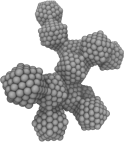
\includegraphics[width=\textwidth]{figs/particle_transparent.pdf}
      \column{0.5\textwidth}
      \centering
      \includegraphics[width=\textwidth]{figs/CB_Image.jpg}
      {\scriptsize Medalia. Rubber Chem. Technol. 47, 411 (1974)\par}

    \end{columns}
    }
  \end{columns}
% }}}
\end{frame}

\begin{frame}[c]{Extensional deformation molecular dynamics provides stress response}
% {{{
  \begin{columns}[c]

  \column{0.55\textwidth}
  \centering

%  \vspace{-1\baselineskip}
  \animategraphics[width=\textwidth]{3}{../figures/Neat_Stretching/Neat_Stretching-}{0}{39}

  \vspace{1.0\baselineskip}

  \animategraphics[width=\textwidth]{3}{../figures/Filler_Stretching/Filler_Stretching-}{0}{39}

  \column{0.45\textwidth}
  \centering

  \vspace{\baselineskip}
  \onslide<2>{
  \includegraphics[]{../figures/fig-stress_vs_shear/fig-stress_vs_shear.pdf}
  }

  \vspace{-14.5\baselineskip}
  \onslide<3>{
  \includegraphics[]{../figures/fig-stress_vs_shear/fig-stress_vs_shear.diff.pdf}
  }

  \end{columns}
% }}}
\end{frame}

\begin{frame}[c]{Species--resolved $\sigma$ points to poisson ratio mismatch-driven enforcement}
%Crossover in elastomer reinforcement from 1) by jammed solid at low strain to 2) by plastic granular fluid at high strain}
% {{{
  \begin{columns}[T]

  \column{0.45\textwidth}
  \centering

  \onslide<1->{
  \blocktitle{Tension in x}
  \includegraphics{../figures/fig-stress_vs_shear/fig-stress_vs_shear.groups.pdf}
  }

  \column{0.45\textwidth}
  \centering

  \onslide<2->{
  \blocktitle{Compression in y \& z}
  \includegraphics{../figures/fig-stress_vs_shear/fig-stress_vs_shear.norm.groups.pdf}
  }

  \end{columns}

  \vspace{-\baselineskip}
    {
      \scriptsize 
      Smith and Simmons. Soft Matter. 15, 656 (2019)\par
    }
% }}}
\end{frame}

\begin{frame}[c]{A closer look at filler contributions}
%Crossover in elastomer reinforcement from 1) by jammed solid at low strain to 2) by plastic granular fluid at high strain}
% {{{
  \begin{columns}[T]

  \column{0.45\textwidth}
  \centering

  \begin{equation*}
  \Delta \sigma = \sigma^{\mathrm{Filled}} - \sigma^{\mathrm{Neat}}
  = \sigma - \sigma^{0}
  \end{equation*}
  \onslide<2->{
  \begin{equation*}
  = \sigma_{F} + \sigma_{P} - \sigma^{0}
  \end{equation*}
  }
  \onslide<3->{
  \begin{equation*}
  = \bar{\sigma}_{F}x_{F} + \bar{\sigma}_{P}(1-x_{F}) - \sigma^{0}
  \end{equation*}
  }
  \onslide<4->{
  \begin{equation*}
  \Delta \sigma =
  \end{equation*}
  \begin{equation*}
  \left( \bar{\sigma}_{F}-\bar{\sigma}_{P} \right) x_{F} \ \ + \ \ \Delta \bar{\sigma}_{P}
  \end{equation*}
  }

  \onslide<4->{\begin{tikzpicture}

  \node[text width=2.7cm, align=center, fill=white, rounded corners=0.2cm, 
        draw=blue, opacity=0.7, text opacity=1, 
        above right = -1.0 and -2.8, anchor=center] (B) {
    \small{}\color{blue}Direct excess filler contribution\par
  };

  \node[text width=2.7cm, align=center, fill=white, rounded corners=0.2cm, 
        draw=red, thick, opacity=0.7, text opacity=1,
        above right = 0.0 and 4.0 of B.south west, anchor=south west] (C) {
    \small{}\color{red}Filler-modified polymer response\par
  };

  \end{tikzpicture}}

  \column{0.45\textwidth}
  \centering

%  \blocktitle{Compression in y \& z}
  \includegraphics<5->{../figures/fig-component_analysis/fig-component_analysis.pdf}

  \end{columns}
% }}}
\end{frame}
\begin{frame}[c]{Impact of heterogeneity due to particle contact \& interfiller polymer?}
% {{{
  \begin{columns}[T]

  \column{0.45\textwidth}
  \centering

  \begin{tikzpicture}
    \node[ fill, color=red, text=white, rounded corners, inner sep=4pt,
           align=center, minimum width=3cm, minimum height=\baselineskip
    ] 
    {\large Interfiller Polymer\par};
  \end{tikzpicture}
  \includegraphics[height=0.33\textheight]{figs/GlassyBridges.png}

  \vspace{0.5\baselineskip}

  \begin{tikzpicture}
    \node[ fill, color=blue, text=white, rounded corners, inner sep=4pt,
           align=center, minimum width=3cm, minimum height=\baselineskip] 
    {\large Filler Contact\par};
  \end{tikzpicture}

  \includegraphics[height=0.3\textheight]{figs/FillerContact.png}

  \column{0.45\textwidth}
  \centering

  \onslide<2>{
  \blocktitle{Extensional Stress}
  \includegraphics{../figures/fig-pxx_between/fig-pxx_between.groups.pdf}
  }

  \end{columns}

% }}}
\end{frame}

\begin{frame}{Particle--particle contact is particularly important at high temperature}
% {{{
  \begin{columns}[T]

  \column{0.45\textwidth}
  \centering

  \blocktitle{Extensional Stress}
  \includegraphics{../figures/fig-pxx_between/fig-pxx_between.groups.pdf}

  \column{0.45\textwidth}
  \centering

  \blocktitle{Normal Pressure}
  \includegraphics{../figures/fig-pyy_between/fig-pyy_between.groups.pdf}

  \end{columns}
% }}}
\end{frame}

\begin{frame}[c]{Higher temperature of contacting particle shells suggests higher dissipation in contcting filler}
% {{{
  \begin{columns}[T]

  \column{0.45\textwidth}
  \centering

  \vspace{-0.5\baselineskip}
  \begin{tikzpicture}
    \node[ fill, color=red, text=white, rounded corners, inner sep=4pt,
           align=center, minimum width=3cm, minimum height=\baselineskip
    ] 
    {\large Interfiller Polymer\par};
  \end{tikzpicture}
  \includegraphics[height=0.33\textheight]{figs/GlassyBridges.png}

  \vspace{0.5\baselineskip}

  \begin{tikzpicture}
    \node[ fill, color=blue, text=white, rounded corners, inner sep=4pt,
           align=center, minimum width=3cm, minimum height=\baselineskip] 
    {\large Filler Contact\par};
  \end{tikzpicture}
  \includegraphics[height=0.3\textheight]{figs/FillerContact.png}

  \column{0.45\textwidth}
  \centering

  \includegraphics{../figures/fig-temp_between/fig-temp_between.bar.pdf}

  \end{columns}

  \begin{tikzpicture}[remember picture, overlay]
    \node[text width=8cm, align=center, anchor=south east] at ([xshift=-2.0cm,yshift=-0.1cm] current page.south) {
      \small \textcolor{FigPurple}{*\textbf{Preliminary results}}\par
    };
  \end{tikzpicture}

% }}}
\end{frame}

\begin{frame}{Species-- \& spatially--resolved data are insightful}
% {{{
  \begin{columns}[T]

  \column{0.6\textwidth}
  \centering

  \begin{block}{Multiple regimes of reinforcement}
  \begin{itemize}
    \item Jammed solid reinforcement at low $\gamma$
    \item Plastic granular fluid at high $\gamma$
  \end{itemize}
  \end{block}

  \begin{block}{Species-- \& Spatially--resolved data}
  \begin{itemize}
    \item Higher temperature in filler during extension
    \item Particle--particle contact is origin of reinforcement at high T
  \end{itemize}
  \end{block}

  \begin{block}{How general are these results?}
  \begin{itemize}
    \item What happens at low T? Glassy bridges?
    \item Effect of dispersion state, cluster size, etc.?
    \item Filler--filler \& filler--polymer interactions
  \end{itemize}
  \end{block}

  \column{0.40\textwidth}
  \centering

  \includegraphics[]{../figures/fig-stress_vs_shear/fig-stress_vs_shear.ratio.pdf}

  \includegraphics[]{../figures/fig-pratios_between/fig-pratios_between.ratio.pdf}

  \end{columns}
% }}}
\end{frame}

\begin{frame}[t]{Acknowledgements}
% {{{

  \begin{columns}[T]

    \column{0.75\textwidth}
      \centering
      \begin{tikzpicture}

        \node[text width=\columnwidth, align=center, inner sep=0pt] (A) {
          %\includegraphics[width=\textwidth]{figs/Simmons_Group_Picture.jpg}
          \includegraphics[trim={30 200 200 100}, clip, width=\textwidth]{figs/2023_Simmons_Group.jpg}
        }; 

        \node[text width=1.5cm, align=center, fill=white, rounded corners=0.2cm, 
              opacity=0.5, text opacity=1, 
              above right = 5.0 and 4.8 of A.south west, anchor=south west] (B) {
          \small{}David S. Simmons\par
        };

        \node[text width=1.5cm, align=center, fill=white, rounded corners=0.2cm, 
              draw=lightorange, thick, opacity=0.5, text opacity=1,
              above right = 2.5 and 5.8 of A.south west, anchor=south west] (C) {
          \small{}Harshad Bhapkar\par
        };

      \end{tikzpicture}

    \column{0.25\textwidth}
%      \vspace{-8pt}
%      {\small
%      \begin{itemize}
%        \item {\color{lightorange}Prof. Glenn Fredrickson (UCSB)}
%        \item Prof. Hector Ceniceros (UCSB)
%        \item {\color{lightorange}Dr. Kris Delaney (UCSB)}
%        \item Dr. Tatsuhiro Iwama (Asahi Kasei)
%        \item {\color{lightorange}Jan Garcia (UCSB)}
%      \end{itemize}
%      }
  \begin{tikzpicture}

    \node[inner sep=0pt, align=center ] (A)
    { 
%      \includegraphics[width=2.55cm]{./figs/BYU_IM26b.pdf}
      \includegraphics[keepaspectratio, height=0.7in, trim={30 220 30 220}, clip]{../figures/logos/University-of-South-Florida-Symbol.png}
    };

    \node[inner sep=0pt, align=center, anchor=center, below=9 pt of A.south] (B)
    { 
      \includegraphics[height=0.95in]{../figures/logos/DOE_LOGO.png}
    };

    \node[inner sep=0pt, align=center, text width=3cm, below= 3 pt of B.south] (C) { 
      USF CIRCE \\[2pt]
      \includegraphics[height=0.7in]{./figs/BYU_ORC_chassis.jpg}
    };

  \end{tikzpicture}

  \end{columns}
%  \vspace{12pt}
%  \begin{center}
%  \end{center}

% }}}
\end{frame}

\begin{frame}[c]{Different mechanisms of elastomer reinforcement at low and high strain}
% {{{
  \begin{columns}[T]

  \column{0.45\textwidth}
  \centering

  \only<1>{
  \blocktitle{Low $\gamma$}
  }
  \only<2-3, 6>{
  \blocktitle{Jammed Filler Reinforcement at Low $\gamma$}
  }
  \includegraphics<1-3, 6>{../figures/fig-stress_vs_shear_lowgamma/fig-stress_vs_shear.pdf}

  \only<4,5>{
  \blocktitle{Analysis by group}
  \includegraphics<4>{../figures/fig-stress_vs_shear/fig-stress_vs_shear.groups.pdf}
  \includegraphics<5>{../figures/fig-stress_vs_shear/fig-stress_vs_shear.diff.pdf}
  }

  \column{0.45\textwidth}
  \centering

  \only<1>{
  \blocktitle{High $\gamma$}
  }
  \only<4->{
  \blocktitle{Plastic Granular Fluid at High $\gamma$}
  }
  \only<1,4->{
  \includegraphics{../figures/fig-stress_vs_shear/fig-stress_vs_shear.pdf}
  }

  \only<2,3>{
  \blocktitle{Analysis by group}
  \includegraphics<2>{../figures/fig-stress_vs_shear_lowgamma/fig-stress_vs_shear.groups.pdf}
  \includegraphics<3>{../figures/fig-stress_vs_shear_lowgamma/fig-stress_vs_shear.diff.pdf}
  }

  \end{columns}
% }}}
\end{frame}

\end{document}
